% Created 2015-03-03 Tue 17:17
\documentclass[12pt, a4paper]{article}
\usepackage[utf8]{inputenc}
\usepackage[T1]{fontenc}
\usepackage{fixltx2e}
\usepackage{graphicx}
\usepackage{longtable}
\usepackage{float}
\usepackage{wrapfig}
\usepackage{rotating}
\usepackage[normalem]{ulem}
\usepackage{amsmath}
\usepackage{textcomp}
\usepackage{marvosym}
\usepackage{wasysym}
\usepackage{amssymb}
\usepackage{hyperref}
\tolerance=1000
\usepackage{fullpage}
\usepackage{graphicx}
\usepackage{authblk}
\usepackage{mathtools}
\usepackage{setspace} % for adjusting TOC line spacing
\usepackage{algorithm} % typesetting algorithms
\usepackage{algpseudocode} % typesetting algorithms
\renewcommand{\algorithmicrequire}{\textbf{Input:}}
\setlength{\parindent}{0pt}
\setlength{\parskip}{1em}
\setlength{\affilsep}{0.5em}
\usepackage[backend=bibtex,sorting=none]{biblatex}
\usepackage{hyperref}
\addbibresource{refs_supplement.bib}
\newcommand{\LH}{\mathcal{L}}
\author[1]{Aleksandra Vancevska}
\author[1]{Verena Pfeiffer}
\author[2]{Kyle M. Douglass}
\author[1]{Joachim Lingner}
\author[2]{Suliana Manley}
\affil[1]{Swiss Institute for Experimental Cancer Research (ISREC), EPFL, Lausanne, Switzerland}
\affil[2]{Institute of Physics of Biological Systems, EPFL, Lausanne, Switzerland}
\date{}
\title{Supplementary Material}
\hypersetup{
  pdfkeywords={},
  pdfsubject={},
  pdfcreator={Emacs 24.4.50.1 (Org mode 8.2.6)}}
\begin{document}

\maketitle
\setcounter{tocdepth}{2}
\tableofcontents

\begin{abstract}
This is the supplementary material accompanying the manuscript.
\end{abstract}

\section{Telomere size determination from STORM data}
\label{sec-1}

\subsection{Data acquisition}
\label{sec-1-1}
Fixed Hela cells containing Cy5-labeled telomeric DNA were imaged
on an inverted Nikon N-STORM microscope with a 100x/1.49 N.A. Nikon
APO TIRF objective and an Andor iXon3 897 EMCCD camera. Two lasers,
a 500 mW, 640 nm Coherent Sapphire and 100 mW, 402 nm Coherent
Sapphire were used to induce fluorophore switching and to control
the switching rate, respectively. A cylindrical lens was inserted
between the tube lens and camera to introduce a slight astigmatism
to the microscope's point spread function (PSF). The axial
coordinate of all recorded fluorophore localizations was inferred
from the shape of the astigmatic PSF after a calibration routine
\cite{huang-science-2008}.

For imaging, the camera sensor was cropped to $256 \times 256 \;
   \text{pixels}^2$, corresponding to a $40.96 \times 40.96 \; \mu
   m^2$ field of view (FOV) with a square pixel width equivalent to
$0.16 \, \mu m$ in the sample plane. 10,000 images were recorded
for each FOV. Between 10 and 30 FOV's were recorded for each
experiment. The optimal focal plane position for each FOV was
judged by eye as having the greatest number of in-focus
telomeres. Molecule localization and drift correction was performed
in the Nikon NIS-Elements software, version 4.30.01.

The output of the data acquistion stage of an imaging experiment
consisted of lists of detected molecules with their corresponding
drift-corrected x-, y-, and z-positions. A molecule's measured
position combined with the corresponding precision makes one
localization.

\subsection{Clustering and filtering}
\label{sec-1-2}

\subsubsection{Temporal grouping}
\label{sec-1-2-1}
Fluorescent molecules whose centers appeared in the same pixel for
up to 10 consecutive frames were grouped together as one single
localization \cite{annibale-natmethods-2011}. Fluorescent
molecules that appeared in the same pixel for longer than 10
consecutive frames were removed from the analysis since they could
have likely been from dust or other impurities. This step has the
effects of improving localization precisions of single emitters
that emit for a few camera frames and removing spurious noise
localizations.

\subsubsection{Clustering localizations}
\label{sec-1-2-2}
Localizations in each FOV were sorted into clusters corresponding
to individual telomeres using a Matlab implementation of the
density-based spatial clustering of applications with noise
(DBSCAN) algorithm
\cite{daszykowski-chemometrintelllab-2001}. This algorithm was
applied for two reasons. The first was to group localizations
belonging to different telomeres into distinct clusters. The
second reason was to remove localizations not originating from a
telomere from the dataset.

Briefly, the DBSCAN algorithm first randomly selects a
localization in the dataset and determines whether it has a
minimum number of neighboring localizations, $k$, within a sphere
of radius $\epsilon$ surrounding it. This sphere is called the
``neighborhood'' of the localization. If less than $k$
localizations are identified within the neighborhood, the
localization is labeled as noise and a new point is chosen for
processing.

If, on the other hand, there is a number of other localizations
within the current localization's neighborhood that is greater
than $k$, then a new cluster is started from this point. The
current localization and all points in its neighborhood are added
to the cluster. Then, the localizations within the neighborhoods
of the other points of the cluster are added if they contain at
least $k$ localizations. This process is repeated until all
localizations that are within the cluster are identified. The
process starts again with a new point that is neither noise nor
part of a cluster. Note that localizations that may have been
identified as noise during previous iterations of the algorithm
can be grouped into a cluster. These localizations are located at
the outer regions of individual clusters.

The optimum values for the input parameters to the DBSCAN
algorithm are those that group all localizations from individual
telomeres into separate clusters and that also identify
localizations not belonging to telomeres as noise.

To find the optimum values for the input parameters $k$ and
$\epsilon$, a parameter sweep was performed on the STORM data from
the untransfected Hela L and Hela S experiments. The DBSCAN
algorithm was run on the STORM data from each FOV for a range of
values $\left ( k, \epsilon \right)$. For each pair of values, the
total number of identified clusters was recorded and summed across
all FOV's.

A good pair of values that meets the criteria described above
should lie in an area of the parameter space where there is no
change in the number of identified clusters when the parameters
are varied slightly. The reasoning for this argument is as
follows: if the number of clusters increases as the parameters are
varied, then we are separating clusters of localizations that
would have otherwise been grouped together. On the other hand, if
the number of clusters decreases, then we are combining smaller
clusters that lie very close to one another. Because the
individual telomeres are well-separated, there should be a region
of the parameter space where a small increase in the neighborhood
size or a decrease in the minimum number of points required to
form a cluster \emph{does not} result in the combination of
localizations from separate telomeres into one cluster. Likewise,
because there are a finite number of localizations from a
telomere, there should be a region of the parameter space where a
decrease in the neighborhood size and in the minimum number of
points \emph{does not} result in breaking localizations from a single
telomere into separate clusters.

The number of identified clusters as a function of the input
parameters is shown in Fig. \ref{fig-dbscan-sweep}. Based on this
graph, a minimum number of points per cluster of $k=8$ and a
neighborhood radius of $\epsilon = 65$ was chosen for use in all
analyses in this manuscript, though any pair of values in the area
where the surface is flat would have worked equally well.

\begin{figure}
  \centering
  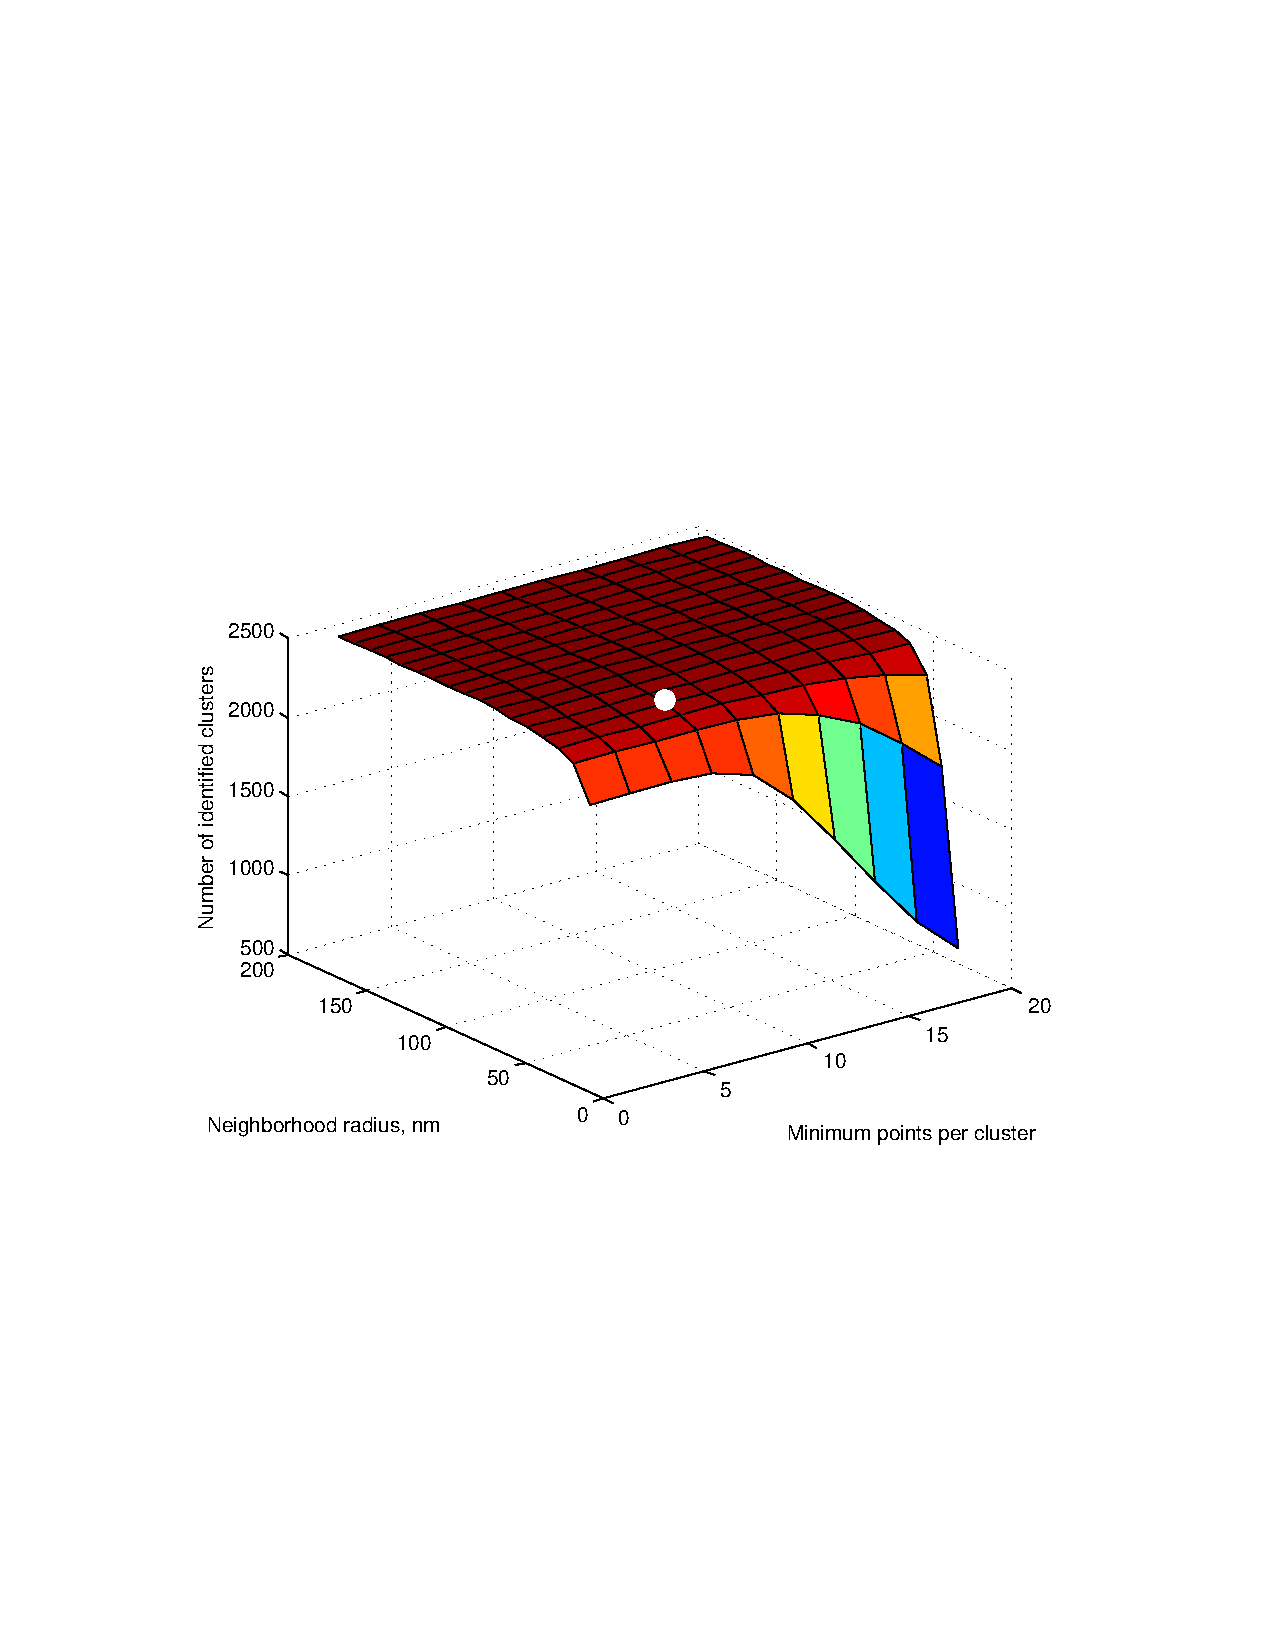
\includegraphics[trim = 0 85mm 0 85mm, clip, scale = 0.6]{fig-dbscan-sweep.pdf}
  \caption{Determining the optimum input parameters for the DBSCAN algorithm. The surface representing the number of identified clusters as a function of the minimum number of localizations per cluster, $k$, and the neighborhood radius, $\epsilon$ is used to find the proper parameter space for isolating single telomeres in the localization datasets. The flat area of the surface where the number of clusters is insensitive to the input parameters indicates a good range of values. The white dot at $\left( k = 8, \epsilon = 65 \right)$ was used for all analyses in this manuscript.}
  \label{fig-dbscan-sweep}
\end{figure}

\subsubsection{Focal volume filtering}
\label{sec-1-2-3}
\label{sec-focalVolumeFiltering}
Axial (z-) coordinates of the localizations were distributed
nonuniformly in the focal volume of the microscope with the
greatest number of localizations identified near the volume's
center transerve plane. Telomeres lying at either extreme of the
axial range of the focal volume may have been truncated due to its
finite extent. Telomeres having a center-of-mass with a
z-coordinate within $100 \; nm$ of the the two extremes were
removed from the analysis to avoid biasing the radius of gyration
distributions. (Note that a shift in the distributions's mean
values of only $\pm 1 \; nm$ was typically observed when filtering
out these extreme telomeres. This indicates that any amount of
bias due to truncated telomeres is very small.)

Clusters that were retained for analysis had axial center-of-mass
coordinates spanning a distance of roughly $600 \; nm$.

\subsubsection{Filtering by number of localizations}
\label{sec-1-2-4}
\label{sec-filter_num_loc}
To ensure sufficient labeling for an accurate determination of the
radius of gyration, telomeres containing fewer than 50
localizations were removed from the analysis. The reason for this
is better explained in Sec. \ref{sec-RgPrecision}. In summary, the
labeling efficiency of a telomere is not 100\%, which means they
are undersampled. Telomere size estimates from fluorophore
localizations are negatively biased by undersampling, and the
magnitude of the bias increases as the number of localizations
decreases.

\subsubsection{Summary of clustering and filtering}
\label{sec-1-2-5}
The grouped, clustered, and filtered localizations were overlayed
with wide field images from the corresponding FOV to ensure that
the clusters corresponded to the individual telomeres and that the
spurious noise in the localization datasets was correctly
eliminated. An example FOV from untransfected Hela L cells with
overlayed and clustered localizations is displayed in
Fig. \ref{fig-widefield-overlay}.

\begin{figure}
  \centering
  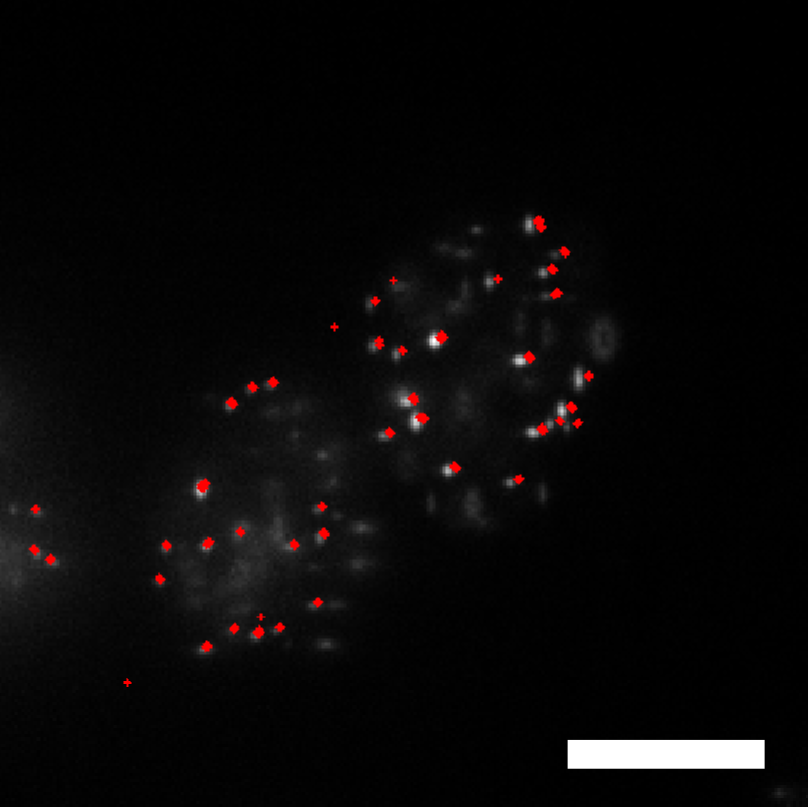
\includegraphics[scale = 0.35]{fig-widefield-overlay.png}
  \caption{A representative widefield image of DNA-FISH labeled telomeres in Hela L cells with localizations belonging to individual telomeres marked in red crosses. Scale bar: $10 \; \mu m$.}
  \label{fig-widefield-overlay}
\end{figure}

\begin{table}[htb]
\centering
\begin{tabular}{|l|p{10cm}|}
\hline
\textbf{Type of clustering/filtering} & \textbf{Parameters used}\\
\hline
Temporal grouping & Keep and group localizations that are on for 10 frames or fewer; Remove localizations on for more than 10 frames\\
\hline
Spatial clustering with DBSCAN & Minimum neighborhood number: $k = 8$; neighborhood size: $\epsilon = 65$\\
\hline
Focal volume filtering & Remove clusters with center of mass z-coordinates outside the range $\left[ -300 \, nm, 300 \, nm \right]$\\
\hline
Removing sparse clusters & Clusters with fewer than 50 localizations per cluster are removed from the analysis\\
\hline
\end{tabular}\caption{Summary of filtering and clustering steps performed on the localization datasets.}

\end{table}

\subsection{The radius of gyration as telomere size}
\label{sec-1-3}

\subsubsection{Definition of the radius of gyration}
\label{sec-1-3-1}
The radius of gyration $R_g$ of a single cluster of localizations
is defined by the following expression:

\begin{equation}
\label{eq-rgSquared}
R_g \coloneqq \left[ \frac{1}{n} \sum_{i = 1}^{n} \left( \mathbf{r}_i - \bar{\mathbf{r}} \right)^{\intercal} \left( \mathbf{r}_i - \bar{\mathbf{r}} \right) \right]^{1/2}
\end{equation}

where $n$ is the number of localizations in the cluster,
$\mathbf{r}_i$ is the vector representing the position of the
$i$'th localization, $\bar{\mathbf{r}}$ is the mean position of
all the localizations, and $\intercal$ is the symbol denoting
vector transpose. Eq. \eqref{eq-rgSquared} is equivalent to the
root-mean-square distance of the localizations from the center of
gravity of the cluster.

The radius of gyration of a linear chain polymer is given by the
same expression as in Eq. \eqref{eq-rgSquared}, except that $n$
becomes the number of Kuhn statistical segments while
$\mathbf{r}_i$ and $\bar{\mathbf{r}}$ represent their individual
positions and mean location, respectively
\cite{flory-statmechchainmolecules-1989}.

In Sec. \ref{sec-RgPrecision} it is empirically demonstrated that
the two different radii of gyration are equivalent to within a
nanometer in the limit that the localization precision goes to
zero and telomeres with fewer than 50 localizations are excluded
from the analysis. In other words, the radius of gyration of the
cluster of localizations is a biased estimator of the radius of
gyration of a telomere's Kuhn statistical segments, and this bias
is less than a nanometer in magnitude. The case of a non-zero
localization precision is treated in Sec. \ref{sec-STORMDatasets}.

Because the localization precision in the z-coordinate is worse
than in the x- and -y directions, $R_g$ values for constellations
of localizations were computed from only the x- and y-coordinates
and multiplied by a factor of $\sqrt{3/2}$ to convert them to a
three-dimensional value \cite{rivetti-jmolbiol-1996}. The
z-coordinate was used for filtering out telomeres close to the
edges of the focal volume in Sec. \ref{sec-focalVolumeFiltering}.

\subsubsection{Reasons for choosing $R_g$ as a measure of telomere size}
\label{sec-1-3-2}
The radius of gyration was chosen as a measure of telomere size
for the following reasons:
\begin{enumerate}
\item The structure of the data from a STORM experiment suggests a
statistical measure of size. The data consists of a
constellation of localizations in space whose positions are
subject to measurement imprecision and which are randomly
located along the telomere fiber.
\item The end-to-end distance of the telomere fiber could not be
determined. This is because there is no way to differeniate
localizations at the ends of the telomeric region of the
chromatin from localizations found somewhere in the middle.
\item The radius of gyration allows for comparison to polymer models.
\item $R_g$ characterizes a cluster of localizations with a single
number while managing to capture some of the cluster's spatial
non-uniformity.
\end{enumerate}

\subsubsection{Labeling efficiency and precision in $R_g$}
\label{sec-1-3-3}
\label{sec-RgPrecision}
Hela S telomeres were around 10 kbp long, while Hela L telomeres
were about 25 kbp in length. Typically, there were about 100 to 200
localizations identified in each cluster of Hela S and Hela L
telomeres, respectively. Given a DNA-FISH oligonucleotide label
length of 18 bp, this means that the labeling efficiency of
telomeres in this study was only about 15\% to 20\%.

Because the labeling efficiency is small, a series of simulations
was performed to assess the accuracy and precision in the estimate
of the telomere mean radius of gyration. 100,000 wormlike chain
conformations were simulated with a packing ratio of $50 \,
    bp/nm$, a persistence length of $50 \, nm$, and a length of $25 \,
    kbp$ as described in Sec. \ref{sec-WLCSimulation}. Each chain was
labeled and then downsampled by randomly and uniformly removing
all but a set number of localizations. The mean and variance of
the radius of gyration estimates as a function of the number of
segments preserved in the downsampling are displayed in
Fig. \ref{fig-downsampling}.

\begin{figure}
  \centering
  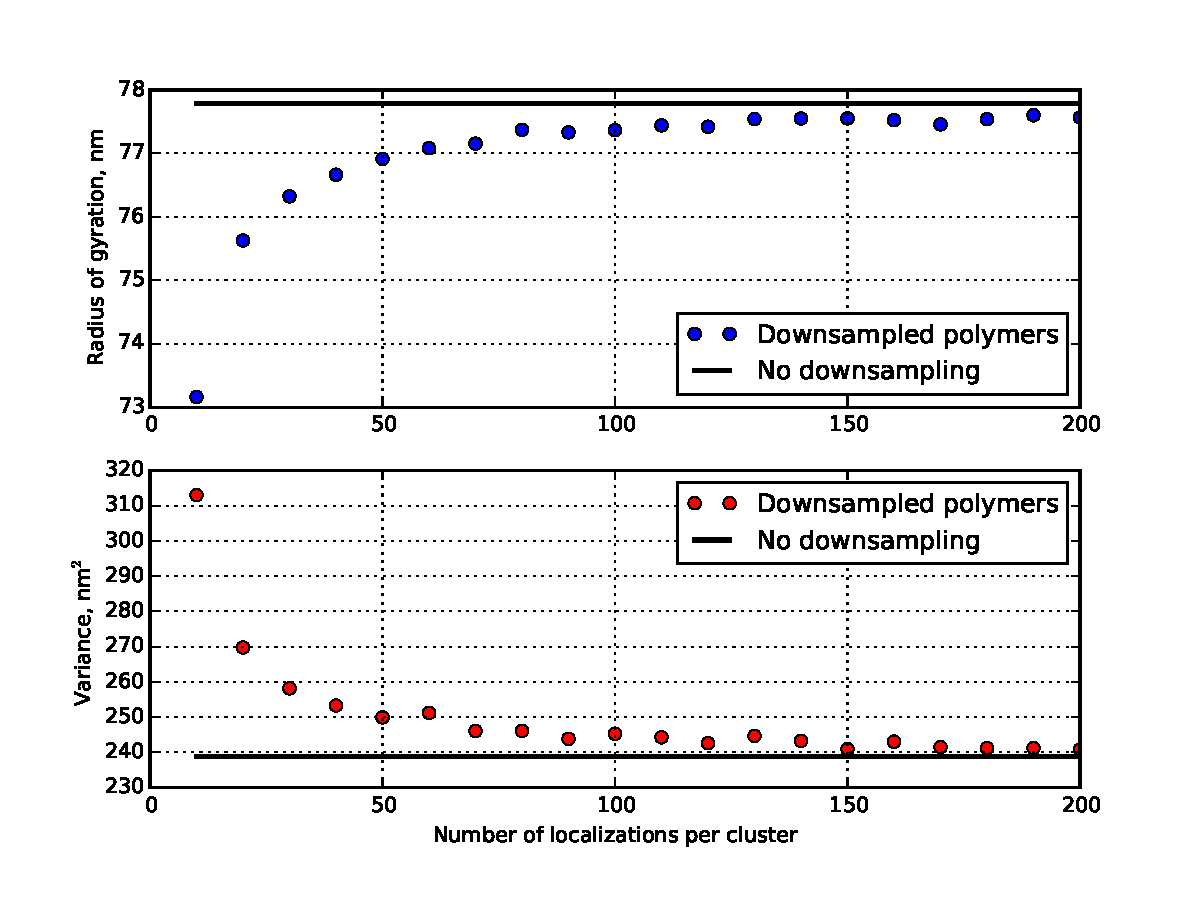
\includegraphics[scale = 0.75]{fig-downsampling_subplots.pdf}
  \caption{The bias in the mean radius of gyration estimate from a constellation of localizations as a function of the number of localizations. This data was generated by simulating 100,000 different polymer conformations and randomly labeling them with fluorophores. The solid horizontal lines denote the values for the fully-labeled polymer. The polymers were generated from an ensemble with a packing ratio of $50 \, bp/nm$, a persistence length of $\ell_p = 50 \, nm$, and a length of $25 \, kbp$.}
  \label{fig-downsampling}
\end{figure}

The results of the simulations presented in
Fig. \ref{fig-downsampling} show that, for the given set of
simulated polymer parameters, telomeres with 50 or more
localizations will have, on the average, $R_g$ values within one
nanometer and a variance in $R_g$ that is less than 5\% of the
real population of telomeres.

In general, the bias should be even less for shorter or more
compact telomeres because they would not require as many labels to
accurately determine their real radius of gyration. For longer or
less compact telomeres, the bias will be worse. The lower cutoff
for filtering clusters based on their number of localizations was
set to 50 in all analyses as discussed in
Sec. \ref{sec-filter_num_loc}. This was chosen as a compromise
between accuracy in determining the radius of gyration by removing
sparsely-labeled telomeres and excluding very small but
well-labeled telomeres in the size distributions.

Another source of error, namely the precision in the location of a
fluorophore, will add an additional bias to the $R_g$
estimate. This bias is taken into account when generating STORM
datasets for performing parameter estimation in
Sec. \ref{sec-STORMDatasets}.

\section{Polymer modeling of STORM datasets}
\label{sec-2}

\subsection{The wormlike chain model}
\label{sec-2-1}
The wormlike chain (WLC) was chosen as the polymer model in this
work because it has been successfully applied in studies of
chromatin conformation at similar genomic length scales as those of
Hela telomeres \cite{bystricky-pnas-2004, huet-2014} and because it
can be easily compared to other models of chromatin packaging, such
as the 10 nm and 30 nm fibers.

The WLC, also known as a Kratky-Porod chain
\cite{kratkyporod-1949}, describes an equilibrium ensemble of
polymer conformations.  In the simplest WLC model, the polymer is
treated as a continuous, semiflexible, and homogeneous rod whose
conformation is deformed by thermal interactions with its solvent
environment. The simple WLC model has a negligible thickness and a
length $L_c$, otherwise known as the contour length. The
flexibility of the rod is described by its persistence length
$\ell_p$. Intuitively, the persistence length is the average length
over which the polymer remains approximately straight. Polymers
with a longer persistence length will be more rigid than shorter
ones.

Mathematically, the persistence length is the characteristic length
describing the exponential decay of the tangent-tangent correlation
function of an infinitely long WLC
\cite{phillips-pbotc-2009, schellman-biopolymers-1974},

\begin{equation}
  \label{eq-tantancorr}
  \left< \mathbf{t} \left( s \right) \cdot \mathbf{t} \left( 0 \right) \right> \sim \exp \left( -s / \ell_p \right)
\end{equation}

where $\mathbf{t} \left( s \right)$ is the unit vector tangent to
the polymer at the one-dimensional coordinate $s$ along the
polymer. For distances $s$ much greater than $\ell_p$, Eq.
\eqref{eq-tantancorr} shows that there will be no correlation in
the direction that the tangent vectors point.

The mean-square radius of gyration of an ensemble of WLC's with the
same contour length and persistence length is \cite{nakamura-2008}

\begin{equation}
  \label{eq-meanWLCRg}
  \left< R_{g}^2 \right> = \frac{2 L_{c} \ell_{p}}{6} - \ell_{p}^2 + \left( \frac{2 \ell_p^3}{L_c^2} \right) \left[ L_c - \ell_p \left( 1 - e^{-L_c/\ell_p} \right) \right]
\end{equation}

In the limit that the contour length $L_c$ becomes much larger than
the persistence length $\ell_p$, Eq. \eqref{eq-meanWLCRg} tends to
$2 L_c \ell_{p}/6$, which is equivalent to the expression for the
mean-square radius of gyration of the freely-jointed chain
(sometimes known as the Gaussian chain) \cite{phillips-pbotc-2009}.

The packing ratio $c$, which describes the linear density of base
pairs per length of the telomere fiber, is related to the contour
length through the simple relation

\begin{equation}
  \label{eq-packingRatio}
  L_c = \frac{n}{c}
\end{equation}

where $n$ is the number of base pairs in the telomere.

\subsubsection{The probability distribution for the bending angle between segments}
\label{sec-2-1-1}

Linear, semiflexible polymers are composed of small molecules and
are thus subject to agitation by the random collisions with
solvent molecules in their environment. These collisions cause the
polymer to adopt one of many random configurations at any given
moment in time. According to Boltzmann's statistics, the
probability that a semiflexible polymer in thermodynamic
equilibrium will bend into of its possible conformations is
proportional to the Boltzmann factor

\begin{equation}
  \label{eq-boltzmann}
  P \left( \Delta U \right) \sim \exp \left( -\frac{\Delta U}{k_B T}\right)
\end{equation}

where $P \left( \Delta U \right)$ represents of the probability of
observing a polymer conformation requiring a free energy change of
$\Delta U$, $k_B$ is Boltzmann's constant and $T$ is the absolute
temperature of the system. The fact that it takes energy to bend
the polymer into a particular conformation reflects the
``semiflexible'' qualities of the polymer.

The energy $U$ of a particular conformation can be approximated by
first discretizing the polymer by dividing it into very short line
segments and determining the local energy associated with the bend
between segments $i$ and $i+1$. The total energy $U$ of the chain
is then the summation of all the local bending energies.

The local bending energy $U_i$ may be Taylor expanded about its
average

\begin{align}
  &U_i = U_{0,i} + \frac{dU_i}{d\theta_i} \theta_{i} + \frac{1}{2} \frac{d^2 U_i}{d \theta_i^2}\theta_i^2 + \ldots \\
  &\Delta U_i \approx \frac{1}{2} U_i'' \theta_i^2 \label{eq-bending-energy}
\end{align}

where terms higher than second order have been dropped and the
constant $U_{0,i}$ has been subtracted from both sides in
Eq. \eqref{eq-bending-energy} to arrive at the change in
energy. The first derivative is zero when the polymer is at
equilibrium
\cite{schellman-biopolymers-1974}. Eq. \eqref{eq-bending-energy}
and Eq. \eqref{eq-boltzmann} can be combined to give the
unnormalized probability distribution function for the bending
angle. If the axis about which the two segments $i$ and $i+1$ bend
is fixed and perpendicular to both segments, then the integration
producing the normalization factor is only over the zenith angle
$\theta$ and the probability distribution for the bending angle
$\theta_i$ is of the form

\begin{equation}
  P\left( \theta_i \right) = \left( \frac{1}{2 \pi \sigma^2} \right)^{1/2} \exp \left( -\frac{\theta_i^2}{2 \sigma^2} \right) \label{eq-gaussianPDF}
\end{equation}

with the variance equivalent to $\sigma_i^2 = k_{B} T/U_i''$. This
model was developed and called the \textit{hinge model} in
Ref. \cite{schellman-biopolymers-1974}; its probability
distribution function for the bending angle is simply a
Gaussian. Letting $s$ now represent the length of a line segment
forming the polymer, the persistence length of the hinge model was
shown to be

\begin{equation}
  \label{eq-pLength}
  \ell_p = 2 s \left( \frac{U_i''}{k_{B} T} \right)
\end{equation}

Substituting Eq. \eqref{eq-pLength} into Eq.
\eqref{eq-gaussianPDF} and using $\sigma_i^2 = k_{B}T/U_i''$

\begin{equation}
  \label{eq-bendingPDF}
  P \left( \theta_i \right) = \left( \frac{\ell_p}{4 \pi s} \right)^{1/2} \exp \left[ -\left( \frac{\ell_p}{4 s} \right) \theta_i^2 \right]
\end{equation}

Eq. \eqref{eq-bendingPDF} is important because it shows that the
bending angle between consecutive line segments is a random number
drawn from a Gaussian probability distribution with a mean of zero
and a variance of $2s / \ell_p$. Gaussian random numbers are
easily generated by computers, so individual WLC conformations can
be simulated using this approach.

\subsection{Wormlike chain simulation}
\label{sec-2-2}
\label{sec-WLCSimulation}
As described in the previous section, a continuous WLC may be
simulated by approximating the chain contour as a series of
discrete line segments of equal length with a random angle between
the line segments drawn from a probability distribution function
given by Eq. \eqref{eq-bendingPDF}.

An extra random variable that describes the orientation of the
hinge axis at each joint is required to simulate a WLC in three
dimensions. This number does not count as a degree of freedom when
determining the form of the probability distribution in
Eq. \eqref{eq-bendingPDF}. If it did, the properties of the
simulated chains would remain the same but the form of the
probability distribution would be modified and the expression for
the persistence length in Eq. \eqref{eq-pLength} would be smaller
by a factor of two \cite{schellman-biopolymers-1974}.

The algorithm for generating a three dimensional WLC based on
these ideas is as follows:

\begin{algorithm}
  \caption{Generating 3D wormlike chains}
  \label{alg-3dWLC}
  \begin{algorithmic}[1]
    \Require{A persistence length $\ell_p$ and a number of segments $N$}
    \Statex
    \State $i\gets 1$
    \State $\mathbf{r}_1\gets \hat{x}$ \Comment{$\mathbf{r}_{1}$ is a unit vector in the x-direction}
    \While{$i \leq N$}
      \State $\theta\gets \text{Gaussian random number with variance equal to } 2/\ell_{p}$
      \State $\mathbf{a}\gets \text{uniformly and randomly oriented unit vector}$
      \Statex
      \While{$\mathbf{r}_i \times \mathbf{a} = 0$} \Comment{Prevents division by zero in a later step}
        \State $\mathbf{a}\gets \text{uniformly and randomly oriented unit vector}$
      \EndWhile
    \Statex
    \State $\mathbf{d}\gets \frac{\mathbf{r}_i \times \mathbf{a}}{\lVert \mathbf{r}_i \times \mathbf{a} \rVert} \left( \sin \theta \right)$ \Comment{$\mathbf{d}$ is perpendicular to $\mathbf{r}_i$}
    \State $\mathbf{r}_{i+1}\gets \mathbf{r}_i \left( \cos \theta \right) + \mathbf{d}$
    \State $i\gets i + 1$
    \EndWhile
    \Statex 
    \State $\text{path} \gets \mathbf{cumsum} \{ \mathbf{r}_i \}$ \Comment{$\mathbf{cumsum}$ is the cumulative summation of a set}
  \end{algorithmic}
\end{algorithm}

This algorithm generates the WLC by generating a random walk on the
surface of the unit sphere. Each point on the walk is represented
by a vector $\mathbf{r}_i$ that points from the origin to the
surface. The orientation of the hinge axis at each joint is
determined by the cross product between the current line segment
and a random vector equally likely to point in any direction. In
the end, the polymer is created by cumulatively summing all the
vectors in the ordered set $\{\mathbf{r}_i\}$ that form the random
walk. The $\times$ operator denotes the vector cross product and
$\lVert \cdots \rVert$ denotes the Euclidean norm of a vector. The
$\gets$ symbol denotes assignment since $=$ is used for testing
equality.

\subsubsection{Accuracy of the simulation}
\label{sec-2-2-1}
The truncation of terms higher than second order in the Taylor
series expansion for the local bending energy in
Eq. \eqref{eq-bending-energy} should result in a small error when
determining the bending angle between segments in this
simulation. This error should get worse as the chain length
increases since each small error will gradually accumulate into a
larger one.

100,000 polymers with different packing ratios were simulated with
a persistence length of $50 \, nm$ and a genomic lengths of $10 \,
    kbp$ and $25 \, kbp$, which roughly correspond to typical lengths
for Hela S and Hela L telomeres. The segment length was set to 2.5
segments per nanometer. In Fig. \ref{fig-simAccuracy} the mean
values of the simulated ensembles as a function of their packing
ratio were subtracted from the theoretical value for $R_g$ given
by Eq. \eqref{eq-rgSquared} to show the bias due to the previously
mentioned approximation. The figure shows that an ensemble of
chains with about 3000 segments, or equivalently a packing ratio
close to $20 \, bp/nm$ with $n = 25 \, kbp$, will have a negative
bias in $R_g$ of about $3 \, nm$ \footnote{The contour length in number of segments is $L_c = nS/c$, where
$n$ is the number of base pairs, $S$ is the number of segments per
nanometer, and $c$ is the packing ratio in $bp/nm$.}. A chain with roughly 6000
segments, for which the packing ratio in this simulation is about
$10 \, bp/nm$ at $n = 25 \, kbp$, will have a negative bias of
about $5 \, nm$.

\begin{figure}
  \centering
  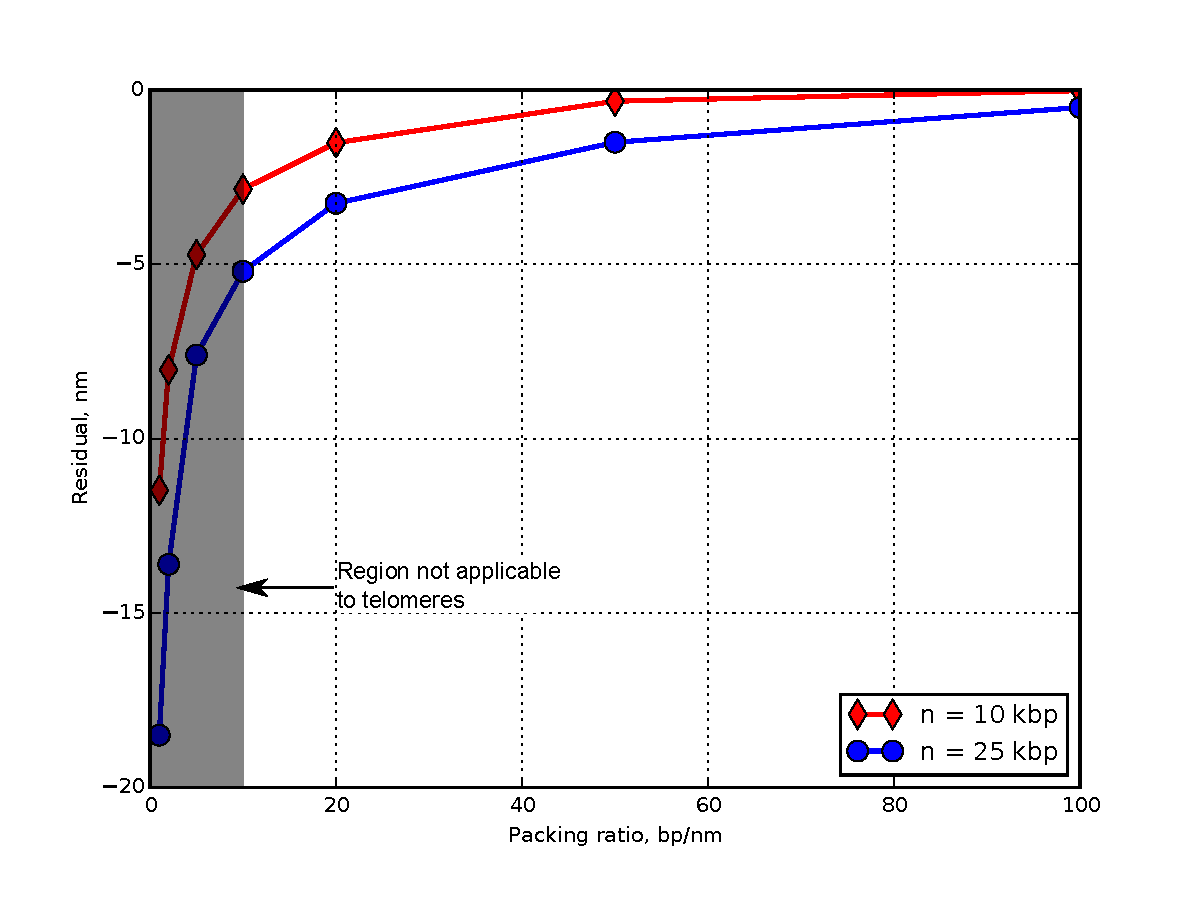
\includegraphics[scale = 0.6]{fig-simulation_accuracy.pdf}
  \caption{The difference between the mean theoretical $R_g$ in Eq. \eqref{eq-rgSquared} and the mean $R_g$ of an ensemble of 100,000 simulated polymers as a function of their packing ratio. The persistence length is $\ell_p = 50 \, nm$ and the number of base pairs was either $10 \, kbp$ or $25 \, kbp$. There were 2.5 segments per nanometer of chain contour in this simulation. The grayed region does not correspond to human telomeres but is included for completeness.}
  \label{fig-simAccuracy}
\end{figure}

The majority of chains in this work were from a region of the
parameter space where the chain length was less than 3000
segments. In the Hela S simulations the number of base pairs was
about $10 \, kbp$ on average, resulting in simulated chains that
are a factor of two to three times shorter.

For these reasons, and taking the results in
Fig. \ref{fig-downsampling} into consideration, the methodology
presented in this manuscript should be adequate for
differentiating between telomere populations with chromatin
packaging models that lead to differences in $R_g$ of a few
nanometers or more when the biases are left uncorrected.

\subsection{Simulating STORM datasets from wormlike chain ensembles}
\label{sec-2-3}
\label{sec-STORMDatasets}
A simulated STORM data set was obtained from the polymer
simulations as follows: First, two values for the packing ratio,
$c$, and the persistence length, $\ell_p$, were chosen from a range
of possible values to test. In this work, the range of values for
$c$ was $\left[ 10 \, bp/nm, 90 \, bp/nm \right]$ and the range of
values for the persistence length was $\left[ 10 \, nm, 200 \, nm
   \right]$

Next, 100,000 WLC conformations were simulated with these
parameters. Each individual chain was assigned a number of base
pairs that was a random number drawn from a uniform probability
distribution. The mean of the distribution was determined from the
peak location in a line profile drawn through the telomere Southern
blot images. The width of the distribution for the number of base
pairs was set to the full width at half maximum of the profile
above the background noise. For Hela L telomeres, the distribution
had a mean of $27 \, kbp$ and a width of $24 \, kbp$, whereas for
Hela S the distribution had a mean of $12.5 \, kbp$ and a width of
$7 \, kbp$. These considerations ensure that the simulated chains
have the same heterogeneity in their lengths as the real telomeres.

\begin{figure}
   \centering
   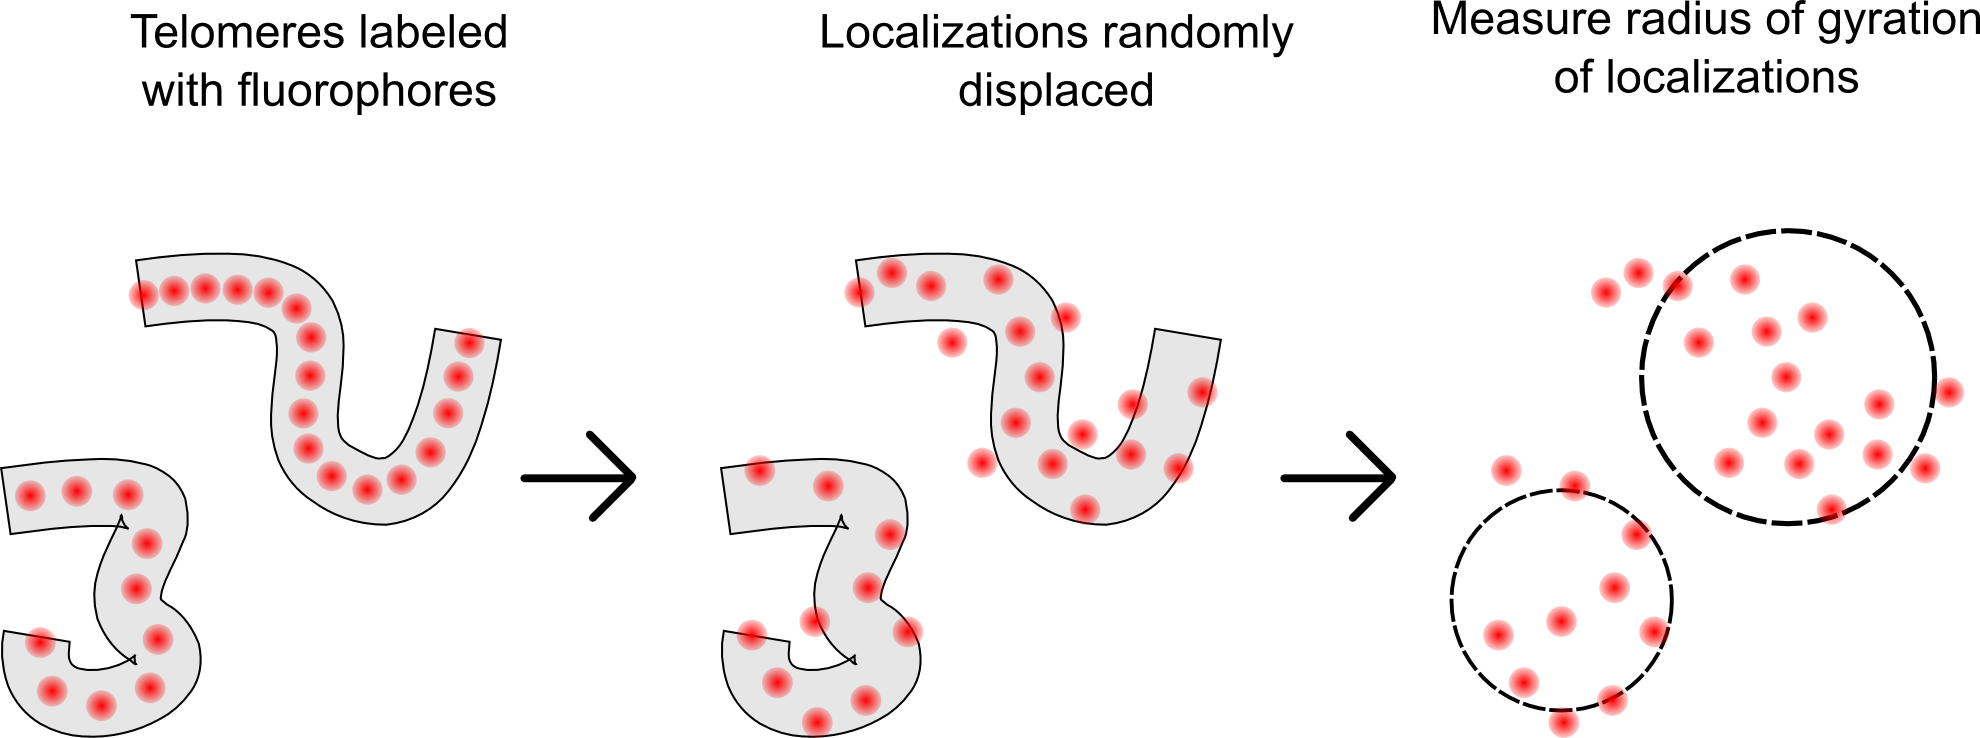
\includegraphics[scale = 1.5]{fig-GenerateSTORMDataset.png}
   \caption{Simulating datasets for comparing to the measured STORM telomere data. WLC conformations were generated and labeled with fluorophores. The fluorophores were randomly displaced to simulate the effects of the imperfect localization precision in the measurement. The radius of gyration was computed from these displaced localizations.}
   \label{fig-GenerateSTORMDataset}
 \end{figure}

Once the polymer conformations were generated, the x-, y-, and
z-coordinates of the endpoints of the segments forming the chain
were randomly bumped by adding a Gaussian random number to each of
them with a mean of zero and a standard deviation equivalent to the
mean localization precision in one transverse dimension. This
reflects the well-known fact in STORM and PALM imaging that the
localized coordinates of a molecule's center are approximately
Gaussian random numbers whose standard deviations decrease with the
number of recorded photons. This idea is illustrated in
Fig. \ref{fig-GenerateSTORMDataset}.

The radius of gyration of the resulting constellation of bumped
points was then computed. The result was one distribution of $R_g$
values of an ensemble of WLC's with parameters $\left( c, \ell_p
   \right)$ and with genomic lengths that reflect the spread in the
real telomere lengths. This process was then repeated for a large
number of different pairs of values for $\left( c, \ell_p
   \right)$. Parameters that led to simulated distributions of $R_g$
values that closely resembled the experimental distributions were
then judged as valid parameters for describing telomere packing and
persistence length. The process of searching for valid parameters
is described in the next section.

\section{Reducing the valid telomere parameter space}
\label{sec-3}
\label{sec-MLE}
The size and less-than-perfect labeling efficiency (see
Sec. \ref{sec-RgPrecision}) makes it impossible to determine the
conformation of any given telomere with STORM in fixed cells. For
these reasons, a statistical forward-problem approach to
determining their packing density and persistence length was
employed in this work.

Simulations of polymer ensembles were generated with different
values for the packing ratio and persistence length. From these
simulated ensembles, distributions of the values for $R_g$ were
computed and compared to the experimental distributions. The
agreement between the measured distributions and the simulated ones,
including the effects of an imperfect localization precision, was
assessed using the likelihood function. The result is a map of the
parameter space of the polymer properties indicating the relative
likelihood that a given set of parameter values produced the
measured data set.

\subsection{The likelihood and log-likelihood functions}
\label{sec-3-1}
The likelihood function is a quantity that is typically used in
maximum likelihood estimation (MLE) for determining best-fit model
parameters. The likelihood function specific to this work is given
by the expression

\begin{align}
  \LH \left( c, \ell_p \mid R_{g,1}, \ldots , R_{g,N} \right) &= P \left( R_{g,1} \mid c, \ell_p \right) \times \ldots \times P \left( R_{g,N} \mid c, \ell_p \right) \\
  &= \prod_{i=1}^{N} P \left( R_{g,i} \mid c, \ell_p \right) \label{eq-LLHProduct}
\end{align}

where $\LH \left( c, \ell_p \mid R_{g,1}, \ldots , R_{g,N} \right)$
is the likelihood that the two parameters for the packing density,
$c$ and the persistence length $\ell_p$ led to the measured dataset
$\left{ R_{g,1} \ldots R_{g,N} \right}$ and $P \left( R_{g,i} \mid
   c, \ell_p \right)$ is the probability of observing a telomere with
radius of gyration $R_{g,i}$ given that the ensemble could be
described by the parameters $c$ and $\ell_p$. The likelihood is
therefore a function of the polymer parameters and computed by
multiplying together the the probabilities of each measured radius
of gyration given the parameters.

Because $N$ is large and the probability of observing any
particular value of $R_g$ is small, the product in
Eq. \eqref{eq-LLHProduct} is too small to compute using typical
floating point data types on computers. Taking the logarithm of
Eq. \eqref{eq-LLHProduct} and working with the log-likelihood
solves this problem. In this case, the product becomes a sum over
all values of the logarithm of the probabilities for $R_g$ but the
analysis remains the same.

\subsection{The likelihood is used to reduce the size of the parameter space}
\label{sec-3-2}
Typically, the maximum of the (log-)likelihood function is used to
find the single set of model parameters that were most likely to
have led to the measured dataset. However, in this work it is used
as a relative measure of how well a simulated distribution of $R_g$
values from a given set of parameters matches the measured set of
$R_g$ values. The reason for this is that a meaningful maximum
value of $\LH \left( c, \ell_p \right)$ doesn't exist because,
depending on the actual size of the telomere, $c$ and $\ell_p$ are
not fully independent parameters for determining $R_g$; $R_g \sim
   \ell_p / c$ when the contour length is much greater than the
persistence length \footnote{This can be seen by allowing the ratio $L_{c}/\ell_p$ to become
very large in Eq. \eqref{eq-meanWLCRg}}.  For this reason, there are multiple pairs
of parameters that are likely to lead to the measured dataset for
small packing ratios.

On the other hand, the packing ratio predominantly determines $R_g$
when the contour length is the same order of magnitude as or less
than the persistence length. There are two reasons for this: the
packing ratio determines the contour length as in
Eq. \eqref{eq-packingRatio} and the telomere is not physically long
enough to measure its persistence length, which is defined in the
limit of an infinite contour length
\cite{schellman-biopolymers-1974}. This explains the sharp, upward
bend in large likelihood values in the parameter space maps where
the log-likelihood becomes independent of $\ell_p$.

Given these considerations, the purpose of this analysis has been
to reduce the size of the parameter space describing the telomeres
so that some models of telomere compaction can be excluded as being
physically likely. An attempt at estimating the exact values for
$c$ and $\ell_p$ has not been made, and is not possible from the
data.

\section{Symbols Abbreviations}
\label{sec-4}
\begin{description}
\item[{DBSCAN}] Density-based spatial clustering of applications with
noise
\item[{FOV}] Field of view
\item[{kbp}] Kilo-base pairs
\item[{PSF}] Point spread function
\item[{$\mathbf{R_g}$}] Radius of gyration
\item[{WLC}] Wormlike chain
\end{description}

\printbibliography
% Emacs 24.4.50.1 (Org mode 8.2.6)
\end{document}
